%Introduction
%\begin{savequote}[50mm]
%If our brains were simple enough for us to understand them, we'd be so simple that we couldn't.
%\qauthor{Ian Stewart }%The Collapse of Chaos: Discovering Simplicity in a Complex World
%\end{savequote}
%[Technologies for interoperable multi-device services]
\chapter{Hybrid broadcast-Internet pilot}
\chaptermark{Deployment}
\label{chap:deployment}

\section{Overview}


The audiovisual sector is undergoing a major transformation due to the emergence of heterogeneous connected devices, including Smart TVs. This reinvention is changing the consumption habits of users, enabling new experiences in which traditional broadcasting and Internet media services are blended. Hybrid broadcast-broadband services build upon on the foundation of standards, such as HbbTV. In this context, this chapter provides details on a large pilot deployment for a multi-device hybrid broadcast-Internet service for a live TV programme. It defines and describes the development and deployment of an innovative live service that EiTB, the Basque public broadcaster, provided to cover the election night in the Basque Country, Spain. This work provides results by showing usage statistics of end-users, and presents a discussion with lessons learned about the current hybrid broadcast-Internet ecosystem and multi-device live services.
%This chapter describes the deployment of a large-scale pilot of a hybrid broadcast-Internet multi-device service for a live TV programme, starting with the hypotheses formulated before the pilot and describing the whole implementation and deployment together with the results and a discussion on the lessons learned.
%
%The main contributions of this work have been:
%\begin{itemize}
%	\item the definition of an innovative hybrid broadcast-Internet multi-device service for a live TV programme, enriching the broadcast with Internet-based content;
%	\item a large-scale pilot deployment of the aforementioned service, carried out with EiTB and based on the implementation of the architecture presented in \cite{Zorrilla2015};and
%	\item the lessons extracted from the experience that allow to obtain some guidelines to improve future implementations and deployments, among others, in terms of multi-device adaptation.
%\end{itemize}

\section{Motivation}\label{questions}
The analysis in Section \ref{hybridEc} shows that there are standards, technologies and solutions that enable the delivery and consumption of live multi-device media services. However, there is not yet a clear methodology, and there are still difficulties in providing a completely self-regulated hybrid services that will work under any circumstances following the COPE paradigm.

In order to find out the causes of the mentioned difficulties, it was decided to build an innovative hybrid broadcast-Internet multi-device service and test it through a large-scale pilot by means of the broadcaster. Prior to the deployment of the large-scale pilot, some questions were identified and answered which would be later checked while working in the real environment:
\begin{enumerate}
	\item \textbf{Question 1: Are broadcast-driven hybrid multi-device services accompanied by a live TV programme interesting for users?} Users might like this kind of applications, since their consumption behaviour is moving towards using more than one device at the same time to learn more about the content they are watching on TV. However, since there are no broadcast-driven hybrid services with a live TV programme, users do not have a reference with which to align their expectations. HbbTV-based applications are typically used for catch-up TV, instead of enhancing broadcast programmes with additional content. Furthermore, at this time, the second screen activity is always performed through an independent application and users are not used to associating different devices in the same session while being in front of the TV. Therefore, in order to make a multi-device service which is related to a live programme successful, users will need a completely usable user interface together with the guidelines on how to use the service.
	\item \textbf{Question 2: Are broadcasters ready to cope with hybrid multi-device experiences?} With broadcasting having always been the unrivalled giant, the environment has changed and now a huge amount of sources are available. Therefore, in order to stay in the game, broadcast technology needs an upgrade, and HbbTV represents a great opportunity. Broadcasters know this and that is why more and more TV channels have their own catch-up HbbTV services.
	
	The problem here is that going ahead with broadcast-driven multi-device experiences for live programmes means a major change in their workflow and business model, and change has never come easily for them \cite{Claudy2012}. Broadcasting has always slowly adopted new technologies, and this is due to the highly regulated environment in which they operate and the time required to achieve a consensus. This regulation also generates a sense of fear of changing to such interactive multi-device experiences, as they would lose the complete control of the environment they have enjoyed until now.
	
	In this context, broadcasters and application developers see the potential of broadcast-driven multi-device services but may feel it is an uncontrolled, unstable, immature and complex technology ecosystem to provide broadcast-driven multi-device services together with a live programme. This holds back the creation of these kinds of services, and that is why they currently limit their HbbTV services to catch-up TV. Probably, they would welcome simplicity in many dimensions if they had to assume these kind of deployments.  
	
	\item \textbf{Question 3: Are HbbTV implementations mature enough for broadcast-driven multi-device services?} HbbTV standard has significantly evolved since its creation in 2009. It has become the interactive TV standard in many European countries, and it has generated movement across the entire globe. HbbTV 1.5 version, published in 2012, brought important improvements over the 1.1 version, which lead to the implementation of a big amount applications, most of the times catch-up TV services. The standard, and its deployment in the market, is mature enough when talking about common single device applications.
	
	HbbTV 2.0 and 2.0.1 versions, published in 2015 and 2016 respectively, brought a powerful toolset including advanced Web technologies towards the interoperability with HTML5 and Companion Screen features, that could completely change the interactive TV towards multi-device services. However, HbbTV 2.0 and 2.0.1 versions are not commercially available at the moment in most of the countries. Therefore, there is still a lack of reference implementation of the standard when talking about multi-device services, leading to disparate HbbTV implementations in TV sets from different manufacturers, even if they have the same HbbTV version. There is also a lack of a certification ecosystem for HbbTV applications, to fully guarantee their compliance.
	
	\item \textbf{Question 4: Are HTML5 and HbbTV convergent enough to solve interoperability problems?} HbbTV has appeared as a standard in order to facilitate the convergence between the Web and TV. However, TV set manufacturers still include heterogeneous Web browsers in their devices, adapting them to HbbTV. Accordingly, they typically include more features defined by W3C than the minimum included in the standard. As illustrated in Figure \ref{fig:hbbtvoverview}, HbbTV 2.0 includes new developments in this HTML5-HbbTV convergence, adding HTML5 features, DOM3 and CSS3. However, it is quite common to find HbbTV 1.0 and 1.5 devices that provide some HTML5 features, even if it is not required by the standard. Furthermore, it is difficult for application developers to find the minimum HTML5 features to provide interoperability with HbbTV and follow the COPE paradigm of one application running in all devices (TV sets but also in laptops and mobiles). Moreover, the mentioned compatibility problems may arise the necessity of making the development as automatic as possible to prevent broadcasters from defining details of implementation and adaptation. 
	\item \textbf{Question 5: Are hardware and processing capabilities of the current TV sets enough to run broadcast-driven hybrid services smoothly?} TV manufacturers might be limiting their TV sets' processing capabilities just to the current needs. The lack of advanced and demanding HbbTV services means that there is no need for excessive processing capabilities. Consequently, this may be leaving the TV set one step behind the rest of devices towards COPE based applications. In this context, efficient implementations may help to bridge the gap between TVs and the rest of devices, at least until this kind of services are more known and attractive. 
	
\end{enumerate}

\section{The innovative hybrid broadcast-Internet multi-device service}\label{usecase}

Election day is a very important event in which more and more information is exchanged. Data, statistics, news, exit polls or social network activity generate a huge amount of content from many different sources that are shared and consumed through different services, applications or devices. 

In this context, EiTB, the Basque Public broadcaster, is the main information source for the election coverage in Basque Country (Spain), offering an up to the minute live TV programme on the night providing the exit polls' results and the official results together with expert debates. Furthermore, they had a Website showing all the data. However, being aware of the fact that elections are a social issue involving millions of people, the broadcaster wanted to go a step further and provide an innovative and interactive service together with the live programme, including additional information.

During the MediaScape research project, a scenario to enhance a Live TV programme with additional content was addressed \cite{D21}, enabling interactivity and personalisation. EiTB was part of the Advisory Board of the project and their interest in the election night, among other use cases, was highlighted since the beginning. MediaScape made it possible to create a first version of the elections prototype, which afterwards evolved into a real pilot once the project ended.

The developed service followed a bidirectional approach. On the one hand, it followed a \textit{Technology push} approach, as the test was used in order to validate on a large scale the libraries developed in MediaScape. For this reason, all the developed functionality was included, resulting in a complex application. Whereas, on the other hand, it was combined with a \textit{Market pull} approach where the broadcaster wanted to provide users an innovative, useful and practical experience to follow the election night in front of the TV.

In greater detail, the service complemented the TV programme with the following content:
\begin{enumerate}	
	\item \textbf{Different cameras} located at the headquarters of the five main parties, all of them providing live streaming.
	\item \textbf{Social network activity} through a list of filtered tweets.
	\item \textbf{Different graphics and tables} showing all the real-time counting data for each part of the region, as they do in their website.
\end{enumerate}

Furthermore, the user had the option to associate the TV to different devices such as smartphones, tablets or laptops, by scanning a QR code or typing in a shared URL. This was possible through a remote server providing a shared state between different devices \cite{Zorrilla2015}, and consequently the devices could be in different networks (e.g. the TV connected to the home Internet gateway and the second screen with 3G/4G. Thus, the application content could be distributed across more than one device being used simultaneously. Finally, all the content could be organised through different templates in each device, giving the user a chance to personalise their experience, both in terms of content and design. Figure \ref{fig:demo} illustrates an example of the use of the implemented service with two users watching different content types working on four devices simultaneously.

\begin{figure}
	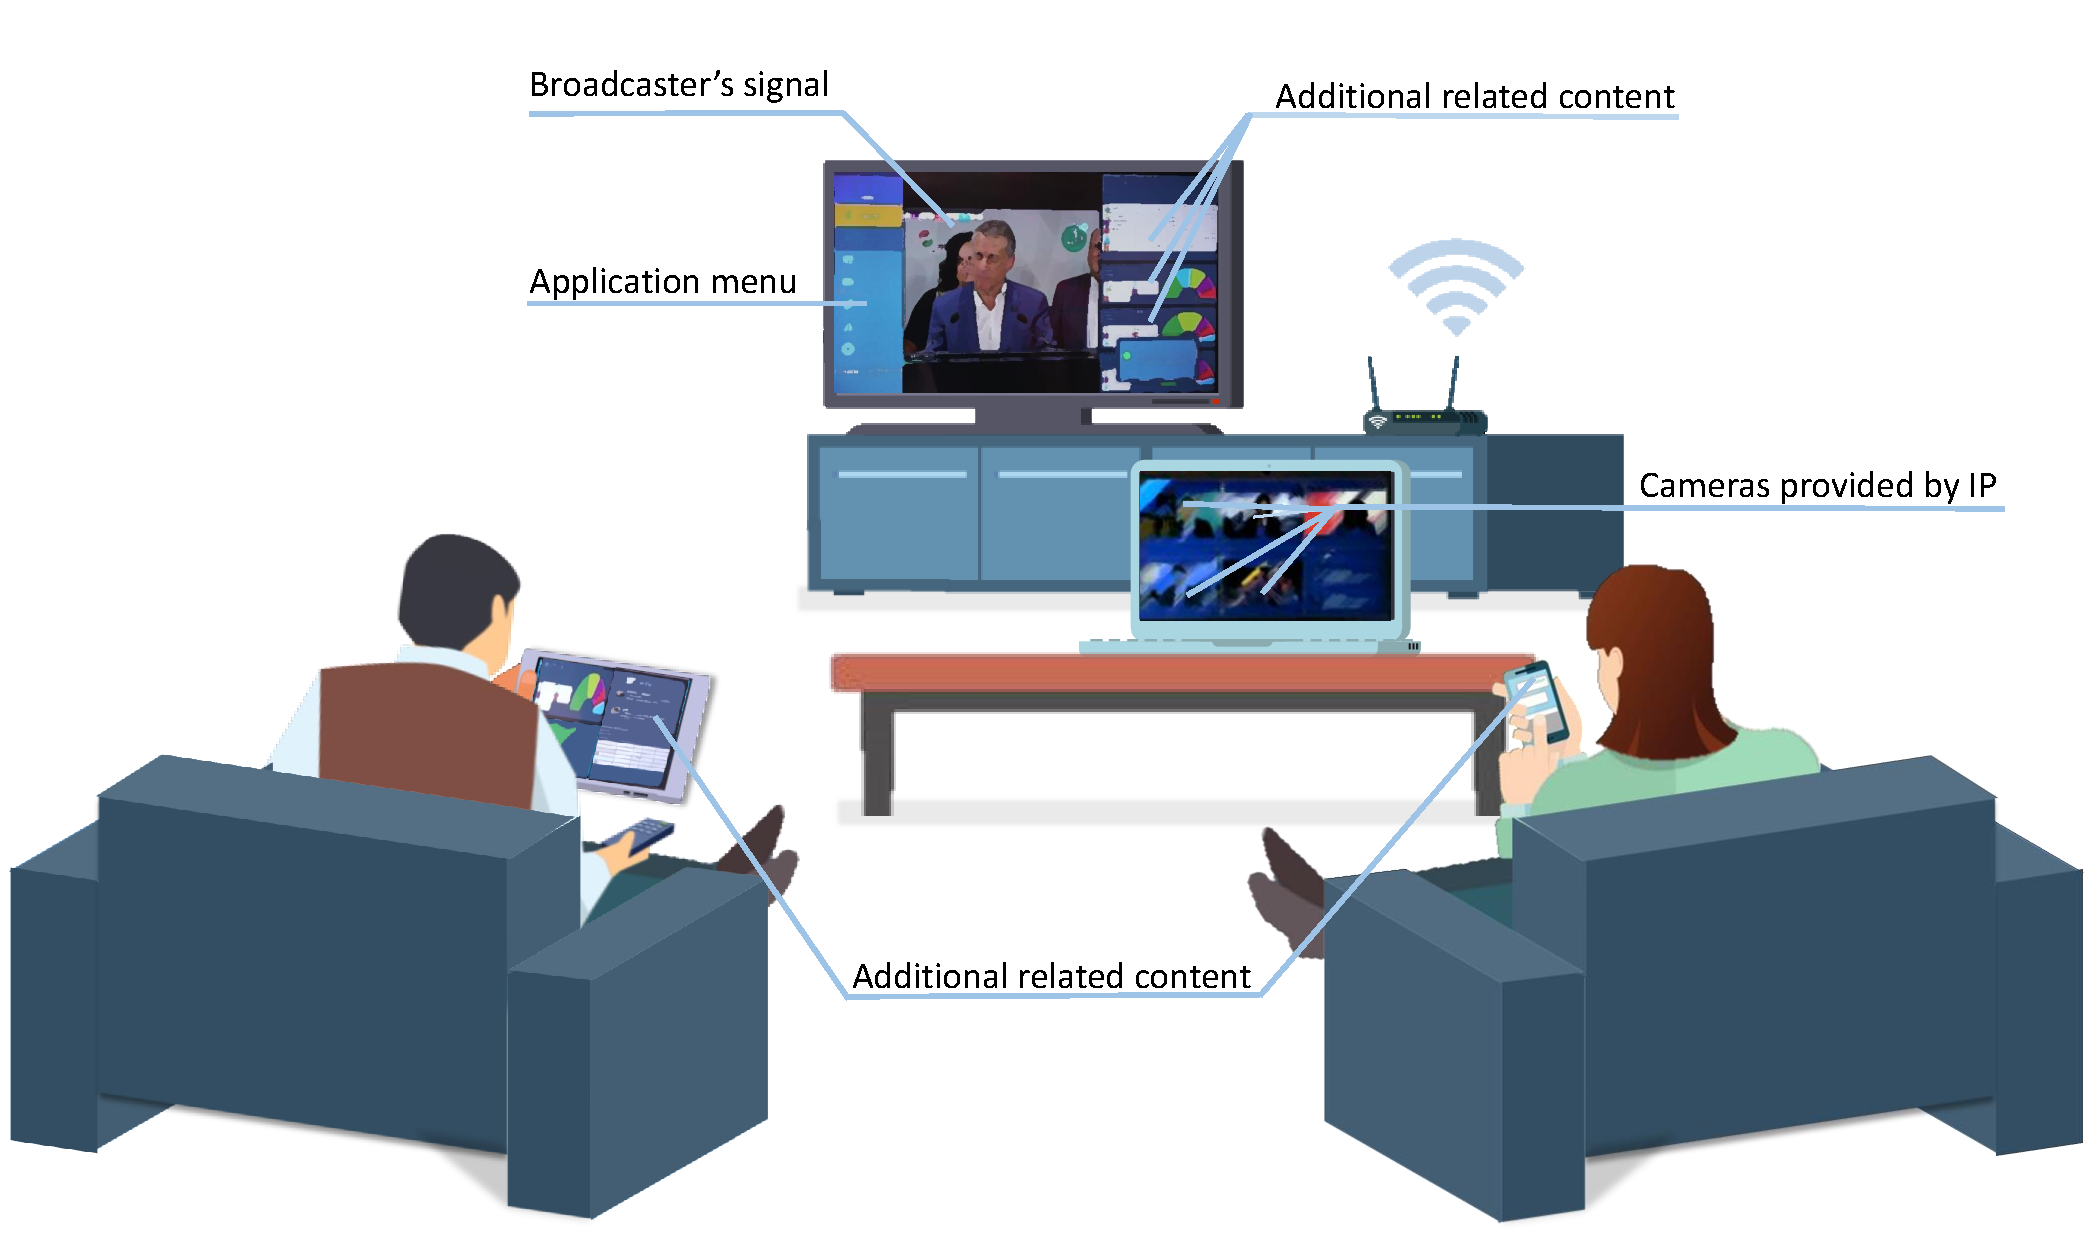
\includegraphics[width=1\textwidth]{usecase_2users_cropped}
	\caption{Application running on four devices simultaneously. In this case, TV and laptop are shared while users interact and personalise the application through their tablet and smartphone. The complete demonstrator can be found in \cite{vimeo}}
	\label{fig:demo}
\end{figure}

Lastly, it is remarkable that although election day is always a very important event for the broadcaster, with one of the highest audiences of the year, they wanted to test the HbbTV multi-device live service, but of course, under some requirements due to all the risks that a live service in which nothing is pre-recorded entails. These requirements are presented in Table \ref{tab:eitbrequirements}.

\begin{table}
	\begin{center}
		\caption{Broadcaster's requirements for the service}\label{tab:eitbrequirements}
		\begin{tabular}{||l|p{10cm}||}
			\hline
			Term & Requirement \\
			\hline
			Access to the service & 
			Access only through the TV as a first device. \\
			&Red button for broadcaster’s official catch-up TV HbbTV service. \\		
			& Blue button for elections application. \\
			& Service available in the two main channels of the broadcaster ETB1 and ETB2.\\ 		
			\hline
			Content template & 
			A layout in which no content overlapped the mainstream. 
			\\
			\hline
			Broadcast always in TV
			& The broadcast always visible in the TV. \\
			& Even if technically possible, access to live streams only through second screens.\\
			\hline
			Control & 
			Every interaction through the second screen also possible through the remote control. \\
			\hline		
			Synchronisation
			&Synchronisation of all content (media sources and data coming from broadcast and Internet) is not critical. \\
			&The broadcaster prefers to follow a best-effort approach of providing all the content when it is ready, rather than introducing a delay on the broadcast to enable synchronisation.\\
			\hline	
			
			Compatibility &   
			Devices having newest browsers, in principle from 2014.			
			\\
			\hline
			Assume little risk  
			& Limited announcement of the service to end-users. \\
			& A management application to control the streaming cameras in real time. The broadcaster would be able to switch on/off of the available cameras during the whole emission, to stop individually each one if required.  
			\\
			\hline
			
			
		\end{tabular}
	\end{center}
\end{table}

\section{Implementation and deployment} \label{architecture}

In this Section we describe the details of the implementation and the real deployment of the interoperable architecture provided in \cite{Zorrilla2015}, that provides a unique and consistent experience across multiple connected devices. For this purpose, the \textit{Created Once and Published Everywhere} (COPE) concept was applied during development by means of standard Web technologies. Therefore, the application was built as an HTML Web page, treating any device (TV set, tablet, smartphone and laptop) as a part of the ecosystem and including the broadcast world simply as a new type of resource. Hence, the application was able to automatically adapt itself to specific target devices, providing the user with a consistent experience through multiple devices at the same time, showing parts of the application on each one of the screens on an adaptive layout.  

The carried out implementation addressed two main scientific challenges described in Chapter \ref{chap:sota} of these kinds of services, such as the device and service discovery described in \cite{zorrilla14bmsb} and \cite{ziegler2013}, and the multi-device adaptation mentioned in \cite{Zorrilla2015}, \cite{zorrilla15bmsb} and \cite{paterno2012}.

Cross device synchronisation was another relevant scientific challenge for hybrid multi-device services \cite{zorrilla2013} \cite{deventer}. The architecture presented in \cite{Zorrilla2015} enables the synchronisation of all the experience using Shared Motion \cite{motion}, and could be easily deployed through the service hosted by Motion Corporation \cite{motioncorp}. However, the synchronisation of all the content (all media sources and data coming from broadcast and Internet) was not critical for the broadcaster in this specific live pilot. Adding synchronisation mechanisms would have required to include a delay in the broadcast content. Instead, the broadcaster preferred to follow a best-effort approach, providing all the content when it was ready (see Table \ref{tab:eitbrequirements} with the requirements of the broadcaster).    

\begin{figure}
	\centering
	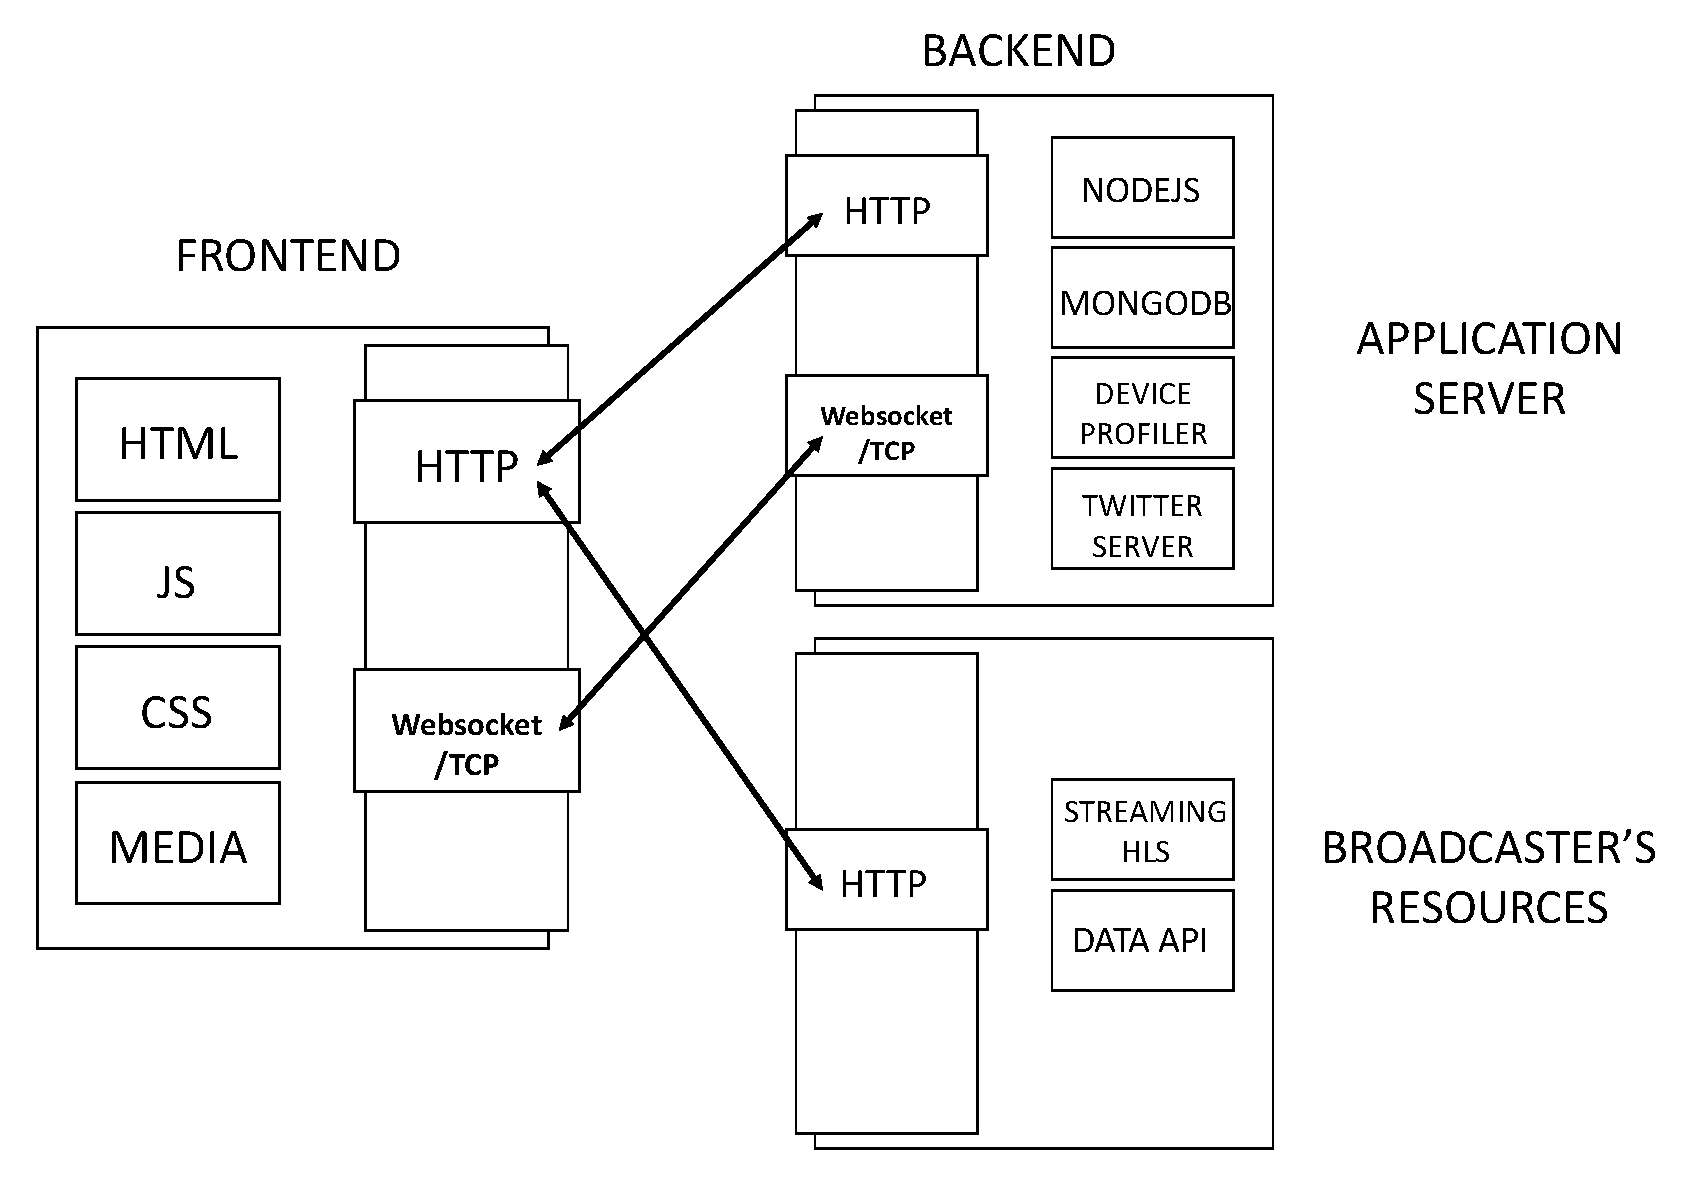
\includegraphics[width=0.8\textwidth]{architecture_cropped}
	\caption{Service implementation}
	\label{fig:appArch}
\end{figure}

Figure \ref{fig:appArch} depicts the service implementation. In the backend side, concerning the service basic structure, three servers and a database were implemented:
\begin{enumerate}
	\item Node.js server: provided all the main Web services and libraries as well as the application specific logic.
	\item Mongo DB database: this was the database in charge of the mapping service, the one which saved all the sessions and shared data and then distributed them correctly among the connected devices. Therefore, it was the one which guaranteed the persistence of the application.
	\item Device Profiler server: in order to detect the type of devices being used in each session or group of devices, with the aim of distributing the elements of the application through them, and basing the decision on an adaptation rule.
	\item Twitter server: responsible for filtering the selected hashtags and accounts from Twitter social network and offering them as a data stream.
\end{enumerate}

Moreover, with regard the application content, the streaming and the necessary counting data for the graphics, these resources were all provided by the broadcaster in real-time by means of five HLS streams and a data API. 

Going through the frontend, the application itself was built on top of standard Web Components \cite{webcomps} to create a Web application in terms of functional elements and therefore, to have the option of distributing and adapting the content across all the connected devices. Web components are a set of Web platform APIs that allow you to create new custom, reusable, encapsulated HTML tags to use in Web pages and Web apps.  

Finally, the communications between frontend and backend were deployed through HTTP and Websockets. 

Concerning the deployment of the servers, the system was scaled in order to cover all the potential users taking into account the initial conditions for the app to work. Referring back to Table \ref{tab:eitbrequirements}, in principle the application could only work on TVs with the latest browsers. Following the broadcaster’s estimates, the number of potential users that could have an HbbTV 1.5 TV (with a newer browser) was 15,000, so the deployment addressed the most challenging (very unlikely situation) scenario where all the potential users access the application concurrently. The deployment of the servers were hosted in Amazon \cite{aws} scaling each server according to its design specifications for the estimated load.

The deployed architecture remained as shown in Figure \ref{fig:scaled} and the characteristics of each one of the nodes correspond with the ones in Table \ref{tab:deployment}.
\begin{table}
	\begin{center}
		\caption{Characteristics of the nodes in the deployment}\label{tab:deployment}
		\begin{tabular}{||l|p{4cm}|c||}
			\hline
			Element & Description & Instances\\
			\hline
			Load balancer & 
			Nginx static file server & 1 \\ 	
			& 8 cpu & \\
			& 1GB of bandwidth & \\
			& 32GB of memory 	&\\
			
			\hline
			Node.js & 
			Xeon server & 1 \\
			& 1 cpu at 2,6 GHz & \\
			& 16GB memory & \\
			\hline
			Mongo DB &  
			Improved SSD until 20,000 operations per second
			& 1\\
			\hline
			Device profiler & 
			Xeon server & 3\\
			& 8GB of memory & \\			
			\hline
			Twitter server & 
			Xeon server & 3 \\
			& 8GB of memory	& \\	 
			\hline
			
		\end{tabular}
	\end{center}
\end{table}
\begin{figure}	
	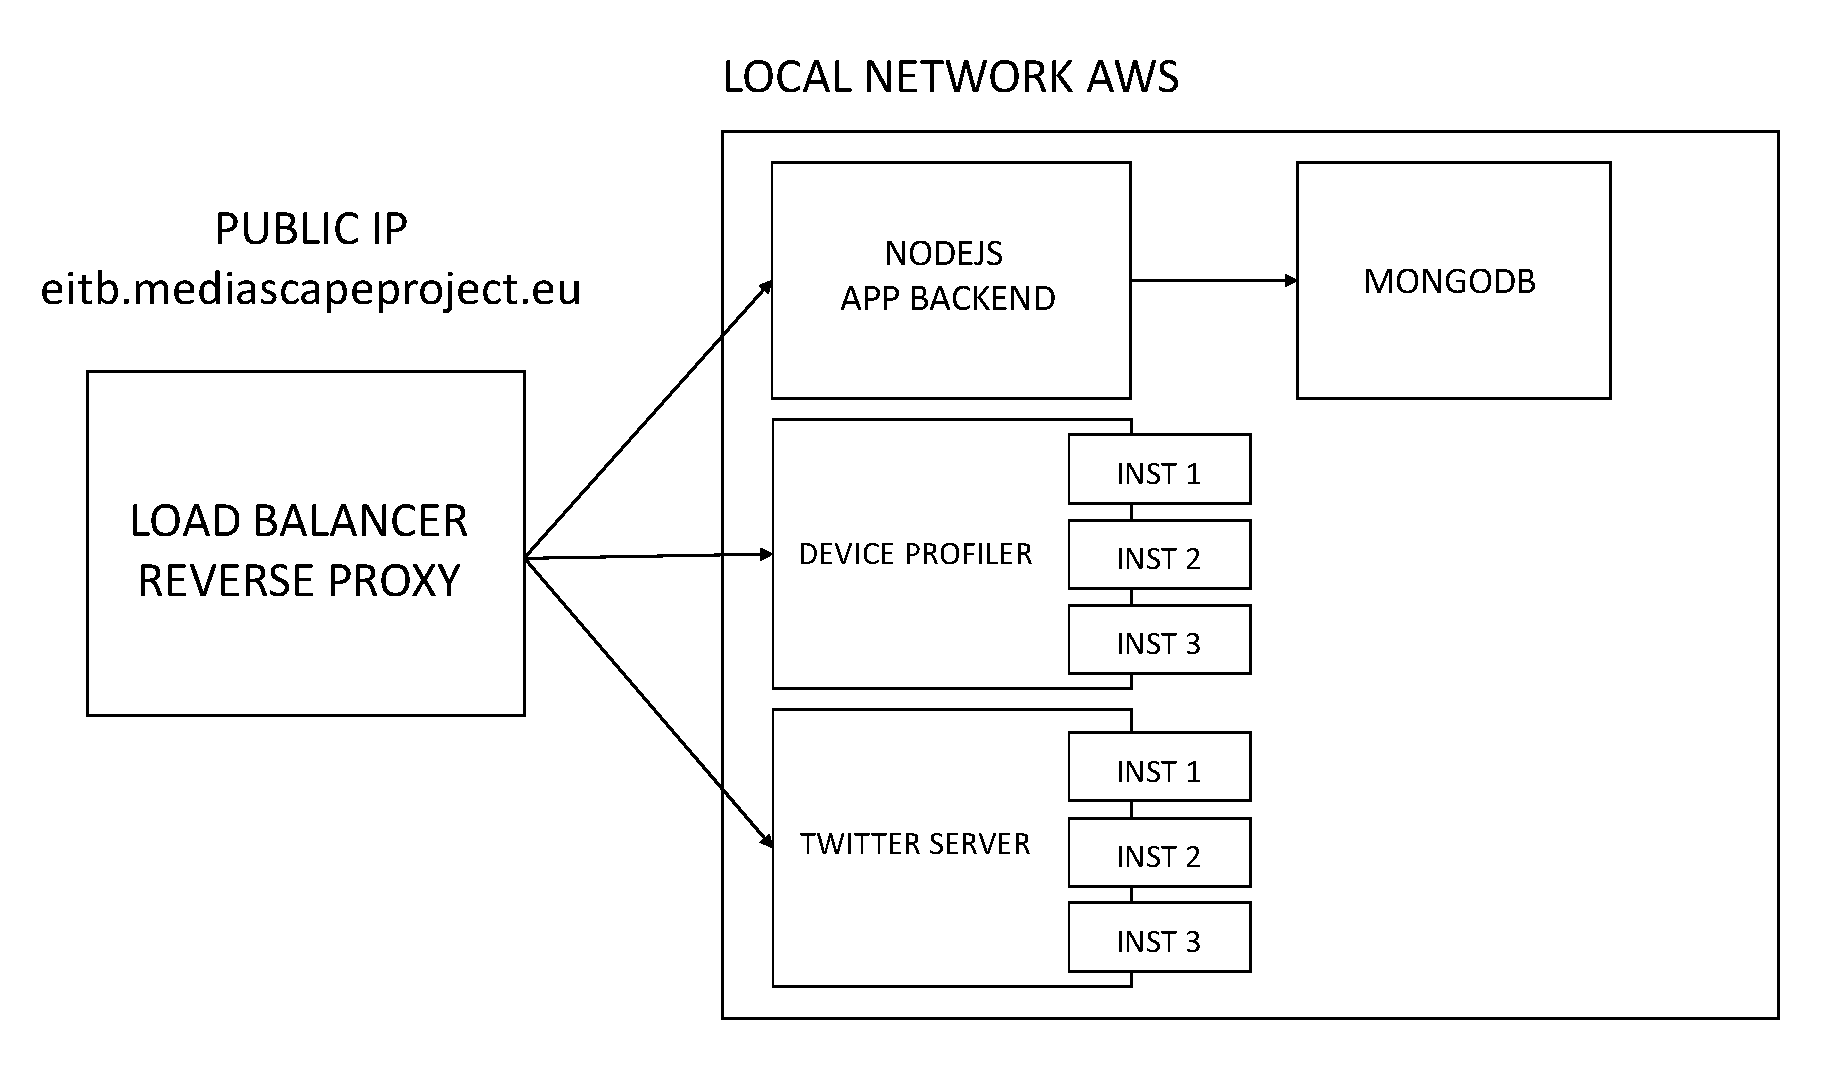
\includegraphics[width=1\textwidth]{scaled}
	\caption{Service deployment in Amazon}
	\label{fig:scaled}
\end{figure}

\section{Results}\label{results}
This section provides a report on the results obtained during the pilot test. All these results have been extracted from the log of the application server, which saved all the User Agent strings of each connected device, and from the analytics modules added both to the Web application and to the servers. The methodology employed has been to analyse all the terms appearing in each User Agent and group all the connected devices according to varying parameters. From this point, the extracted data from the User Agent strings are presented regarding the general terms, the brand, the age of the models, the HbbTV version, the time using the application, the number of sessions and the type of associated devices. Moreover, the results obtained have been compared and contrasted with the data provided by the analytics in order to verify them.  

\subsection{General results} \label{generalres}
As mentioned in Section \ref{architecture}, the amount of concurrent potential users for the service was 15,000. From this point, the presented data correspond to the interval of time between 06:00 pm 25th September 2016, when the server was switched on, and 06:30 am 26th September 2016, when the server was switched off. In that interval, the broadcaster had an audience of 1,161,000, from which 160,000 watched the whole election night TV programme. From this audience, in order to calculate the number of HbbTV devices that received the "press blue button" message, the broadcaster has only the data of HbbTV devices per hour interval. Those data show that the maximum number of devices in the one hour interval was 18,942 from 20:00 to 21:00. Then analysing the rest of the intervals, the estimated total number of single devices was 25,000. Finally, of that number, there were 1,195 users of HbbTV devices who tried to run the application. When classifying the TVs in terms of working or not working devices in the pilot test, the load point in which all the needed files were requested and the content with the main menu was rendered has been taken as a threshold. From this point, when talking about working or not working devices, the mentioned criteria is used. Thus, of the 1,195 users that tried to start the application, 652 devices (55\%) succeeded while 543 (45\%) failed.  

\subsection{HbbTV version}\label{hbbtvres}
Table \ref{tab:hbbtv_tab} shows the summary of the data in terms of the HbbTV version. According to the registered User Agents, of the 1,195 HbbTV connected devices, 82\% were HbbTV 1.5 while 17\% were HbbTV 1.1 and 1\% were HbbTV 2.0. Regarding their performance, a quantum leap is appreciated from HbbTV 1.0 to HbbTV 1.5, increasing the working success by 36 percentage points. Moreover, although HbbTV 2.0 devices were detected through the User Agent string, there are no commercial devices with this version completely implemented, so they could be considered as HbbTV 1.5 devices, as the success rate is almost the same.

\begin{table}
	\begin{center}
		\caption{Hbbtv summary}\label{tab:hbbtv_tab}
		\begin{tabular}{||c|c|c|c|c|c|c||}
			\hline
			\multirow{2}{*}{HbbTV version} & \multicolumn{2}{c|}{Unique sessions} & \multicolumn{2}{c|}{Worked} & \multicolumn{2}{c||}{Failed} \\ \cline{2-7} 
			& Value             & \%               & Value        & \%           & Value          & \%             \\ \hline
			1.0                            & 206               & 17\%             & 51           & 25\%         & 155            & 75\%           \\ \hline
			1.5                            & 974               & 82\%             & 593          & 61\%         & 382            & 39\%           \\ \hline
			2.0                            & 15                & 1\%              & 9            & 60\%         & 6              & 40\%           \\ \hline
			TOTAL                          & 1195              & 100\%            & 652          & 55\%        & 543            & 45\%          \\ \hline
		\end{tabular}
	\end{center}
\end{table}

\subsection{Brands and models}\label{brandres}
Table \ref{tab:brands_tab} shows the summary of the data in terms of brands. As can be seen, there were TVs of many different brands, with the majority belonging to only a few brands. LG was the most used (28\% of users had an LG) and was also the one in which the application worked best (78\% of the LG devices worked). There was also a significant amount of Samsung (25\%), Panasonic (25\%) and Sony (14\%) devices. However, the success percentage decreases in comparison to the LGs, being 54\% for Samsung and Sony, and 38\% for Panasonic.

\begin{table}
	\begin{center}
		\caption{Brands summary}\label{tab:brands_tab}
		\begin{tabular}{||c|c|c|c|c|c|c||}
			\hline
			\multirow{2}{*}{Brand} & \multicolumn{2}{c|}{Single Sesions} & \multicolumn{2}{c|}{Worked} & \multicolumn{2}{c||}{Failed} \\ \cline{2-7} 
			& Value            & \%               & Value         & \%          & Value           & \%            \\ \hline
			LG                     & 332              & 28\%             & 258           & 78\%        & 74              & 22\%          \\ \hline
			Samsung                & 305              & 25\%             & 166           & 54\%        & 139             & 46\%          \\ \hline
			Panasonic              & 294              & 25\%             & 112           & 38\%        & 182             & 62\%          \\ \hline
			Sony                   & 171              & 14\%             & 93            & 54\%        & 78              & 46\%          \\ \hline
			Philips                & 61               & 5\%              & 14            & 23\%        & 47              & 77\%          \\ \hline
			Hisense                & 8                & 1\%              & 4             & 50\%        & 4               & 50\%          \\ \hline
			Other                 & 24               & 2\%              & 5             & 21\%        & 19              & 79\%          \\ \hline
			TOTAL                  & 1195             & 100\%            & 652           & 55\%        & 543             & 45\%          \\ \hline
		\end{tabular}
	\end{center}
\end{table}


\begin{figure}
	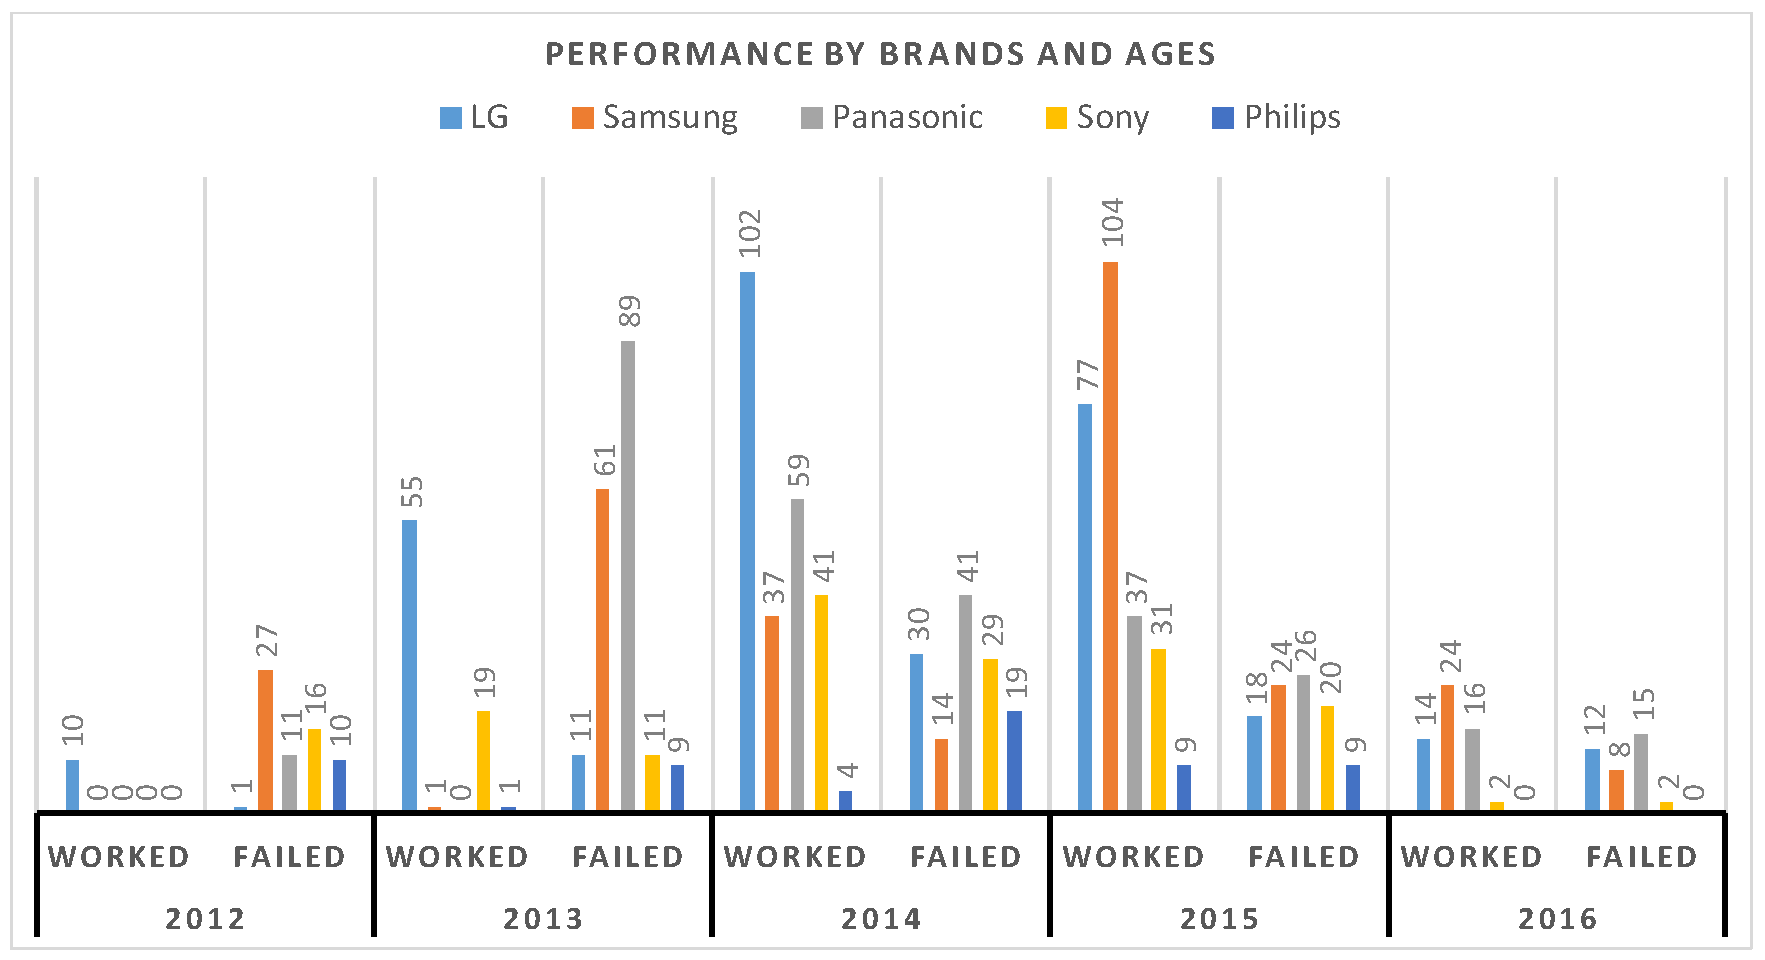
\includegraphics[width=1\textwidth]{brands_years_cropped}
	\caption{Summary of the performance by brands and ages}
	\label{fig:brands}
\end{figure}

On the other hand, Figure \ref{fig:brands} shows the results taking into account the age of the TV models trying to load the application. There were only 7 TVs from 2011 and none of them worked. From 2012, there were more TVs, but most of them did not work. Out of interest, the only working brand was LG. Looking at TVs from 2013, a meaningful increase of the total amount of TVs can be seen. A considerable number of them did not work, but the number of working LGs increased and some Sonys also worked. Most of the models accessing the application were from 2014 and 2015. Looking at 2014, TVs of all brands worked and for the first time, there were more working TVs than not working TVs. Referring back to the broadcaster’s requirement for devices from 2014 or newer, 2015 had the highest number of working TVs. However, for 2016 year there was not enough data to draw conclusions. There were not a lot of TVs and besides, a high percentage of them did not work when the newest models are supposed to work better.

\subsection{Associated devices}\label{associatedres}
As described previously, the user had the option to associate different devices to the TV, creating a unique experience around the TV. Of the 652 working TVs, there were 619 (95\%) users who used only the TV and 33 users who successfully associated another device to the TV. Most of these users, 31 (4.7\%), associated only one device and only 2 (0.3\%) associated two devices.


Table \ref{tab:associated} summarises the type of the mentioned 35 second and third screens, most of them being smartphones and tablets.

\begin{table}
	\begin{center}
		\caption{Type of associated devices}\label{tab:associated}
		\begin{tabular}{||c|c|c|c|c||}
			\hline
			\multicolumn{1}{||c|}{Device}                      & \multicolumn{3}{c|}{Unique sessions} & \%                       \\ \hline\hline
			\multicolumn{1}{||c|}{\multirow{2}{*}{smartphone}} & \multirow{2}{*}{22}    & Android   & 20        & \multirow{2}{*}{62.86\%} \\ \cline{3-4}
			\multicolumn{1}{||c|}{}                            &                        & iOS       & 2         &                          \\ \hline
			\multirow{2}{*}{Tablet}                           & \multirow{2}{*}{11}    & Android   & 7         & \multirow{2}{*}{31.43\%} \\ \cline{3-4} 
			\multicolumn{1}{||c|}{} 			&          
			& iOS       & 4         &   \\ \hline
			Laptop                                            & \multicolumn{2}{c|}{2}             & Windows   & 5.71\%                   \\ \hline
			Total                                             & \multicolumn{3}{c|}{35}                        & 100\%                    \\ \hline
		\end{tabular}
	\end{center}
\end{table}

\subsection{Time spent using application}\label{timeres}
During the same time interval, Figure \ref{fig:tvtimes_a}, Figure \ref{fig:tvtimes_b}, Figure \ref{fig:2stimes} and Figure \ref{fig:sessions} show how long users spent using the application. The time interval scale for these graphs has been chosen according to that used by Google Analytics \cite{analytics} in a parallel analysis. In the case of the TVs, 61\% of the devices stayed connected more than 10 seconds whereas for second screens this percentage was even higher (91\%). So connecting a second screen device may indicate a higher interest in the service. In addition, concerning the TVs, most of the users (75\%) opened the application once, 15\% did so twice and the rest 3 or more times. The same happens with the second and third screens, with 46\% of users connecting once, 31\% twice and the remaining 3 or more times.  

Finally, the maximum number of simultaneous working devices was 54 at 19:24:44. This fact is far from the 15,000 potential concurrent users estimated in the most challenging scenario, thus indicating that the deployment architecture has been under-used. Figure \ref{fig:concurrency} shows the concurrency during the whole time the service was available.

\begin{figure}
	\centering
	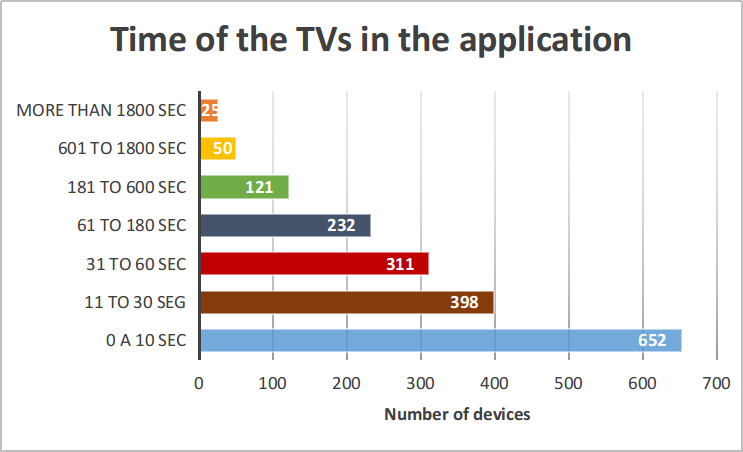
\includegraphics[width=0.8\textwidth]{timestv_a.png}
	\caption{Time spent using the application on TVs classifying the devices along all the different durations.}
	\label{fig:tvtimes_a}
\end{figure}

\begin{figure}
	\centering
	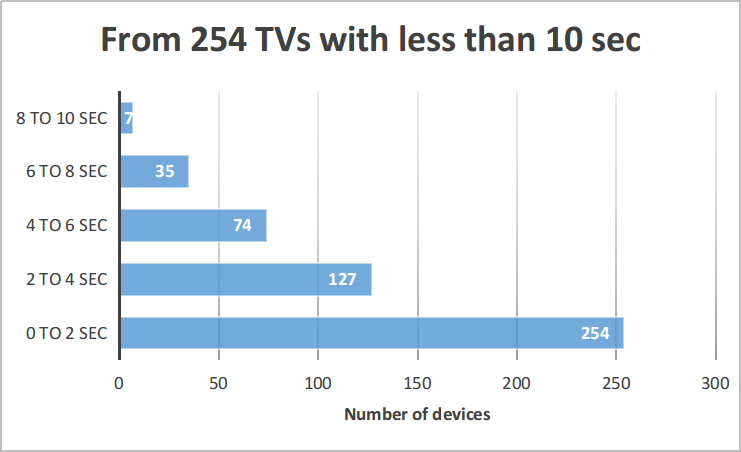
\includegraphics[width=0.8\textwidth]{timestv_b.png}
	\caption{Time spent using the application on TVs showing the detail of the devices being in the application less than 10 seconds.}
	\label{fig:tvtimes_b}
\end{figure}

\begin{figure}
	\centering
	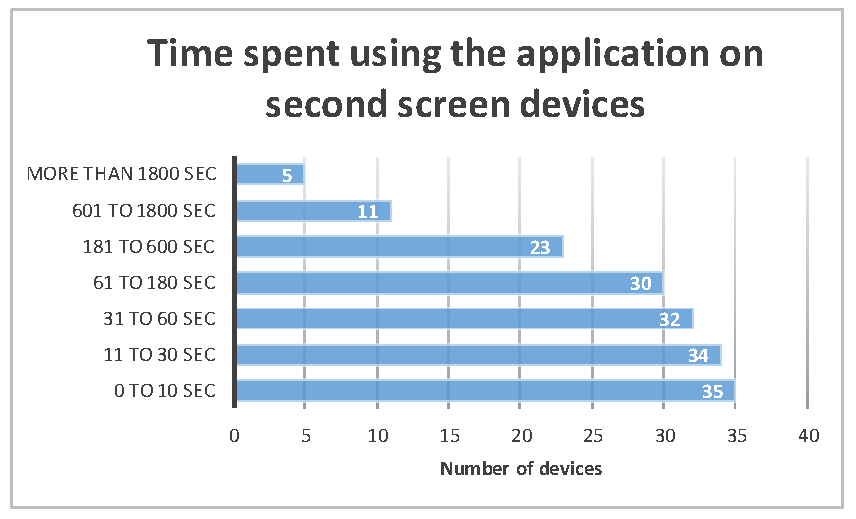
\includegraphics[width=0.8\textwidth]{timesecon_cropped}
	\caption{Time spent using the application on second screen devices}
	\label{fig:2stimes}
\end{figure}

\begin{figure}	
	\centering
	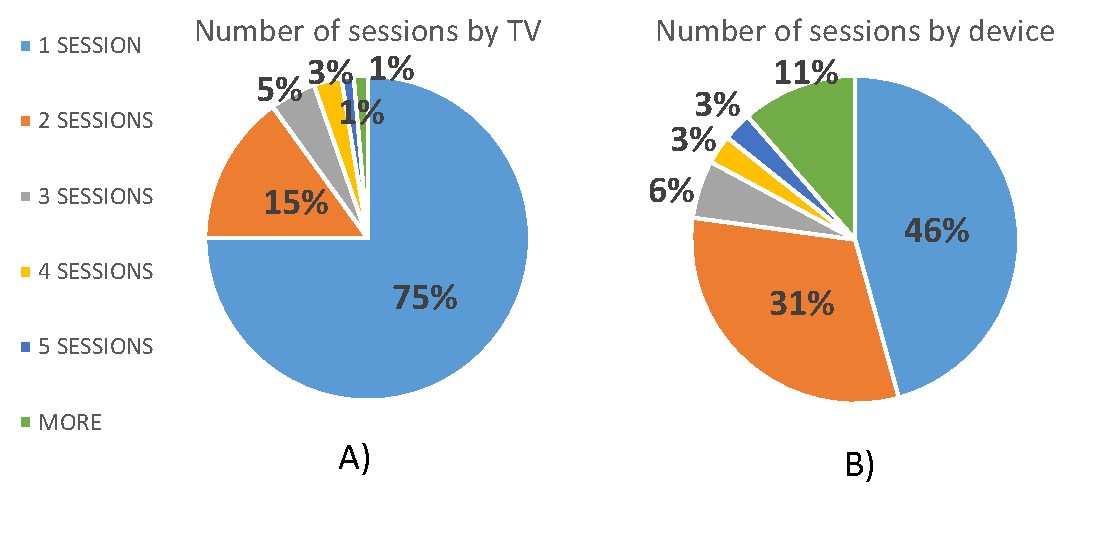
\includegraphics[width=0.8\textwidth]{sessions_cropped}
	\caption{Number of sessions by device. A) Shows the sessions in TVs and B) shows the same data for the rest of devices}
	\label{fig:sessions}
\end{figure}

\begin{figure}
	\centering
	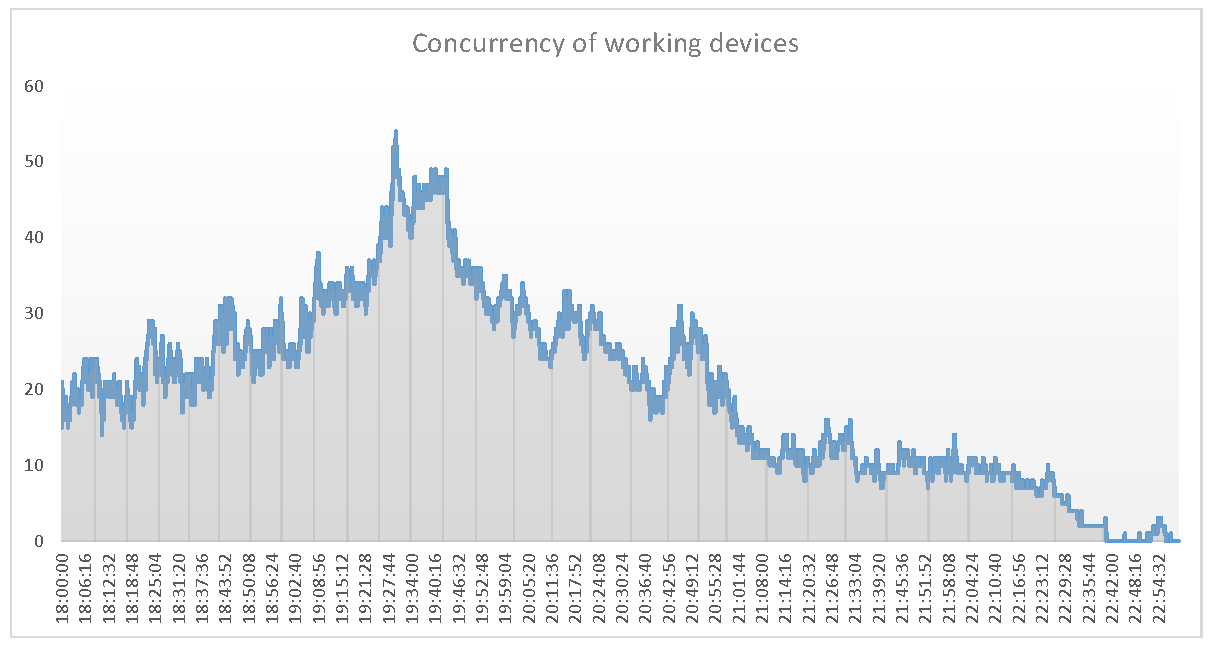
\includegraphics[width=0.8\textwidth]{concurrency_cropped}
	\caption{Concurrency of working devices from 18:00 to 23:00. The data from 23:00 to 06:30 are not shown, as they are negligible.}
	\label{fig:concurrency}
\end{figure}

\section{Discussion and lessons learned}\label{discussion}
Once the obtained results have been presented, this section provides a set of lessons learned with the aim of discussing different aspects of hybrid broadcast-Internet multi-device services. The discussion has been driven by giving answers to the questions formulated prior to the test and presented in Section \ref{questions}. The summary of the lessons learned is provided in Table \ref{tab:learnedlessons}.


\begin{table}
	\begin{center}
		\caption{Summary of lessons learned}\label{tab:learnedlessons}
		\begin{tabular}{||m{5.5cm}|m{7.5cm}||}
			\hline
			\textbf{Question} & \textbf{Lessons learned} \\
			\hline
			1. Are broadcast-driven hybrid multi-device services accompanied by a live TV programme interesting for users? &
			Broadcast-driven hybrid multi-device services with a live TV programme are interesting but still unknown for the users. \\
			\hline
			2. Are broadcasters ready to cope with hybrid multi-device experiences? &
			Broadcasters are aware they have to adapt to new consumption experiences within the new hybrid ecosystem but they still have uncertainties about the technology and business models.  \\
			\hline			
			3. Are HbbTV implementations mature enough for broadcast-driven multi-device services? &
			Although HbbTV provides a set of standards that lay the foundations for hybrid services, it needs to overcome ambiguities in the multi-device field towards a consistent and mature specification.			
			\\
			\hline
			4. Are HTML5 and HbbTV convergent enough yet to solve interoperability problems? 
			&  Despite newer HbbTV versions that increasingly include HTML5 features, current HbbTV commercial devices do not provide complete convergence between HbbTV and HTML5. \\
			\hline
			5. Are hardware and processing capabilities of the current TV sets enough to run broadcast-driven hybrid services smoothly? &
			Hardware and processing capabilities of current TV sets are not powerful enough compared to laptops or smartphones to run broadcast-driven hybrid multi-device services smoothly.
			\\
			\hline
			
		\end{tabular}
	\end{center}
\end{table}

\subsection{Answer to question 1: Broadcast-driven hybrid multi-device services with a live TV programme are interesting but unknown for the users.}
Question 1 formulated that services offering a complete environment like the one described in this chapter should succeed among users, based on the fact that TV consumption habits are moving towards the use of a second screen. However, since there are no broadcast-driven hybrid services for live programmes yet, users do not have a reference on which to base their expectations and they need to know what advantages there are to the service and have guidelines on its use.

The limited variety of offered HbbTV catch-up TV services together with the lack of advertising and user guides does not help and causes a loss of interest among users. There is such a degree of dissatisfaction that, according to the broadcaster, some people call to ask how the "red button message" could be removed. They may see it as a useless, unknown and hardly beneficial service when in fact, it could be just the opposite.

In the pilot test, the service was hardly advertised and even less so presented as an advantageous system to follow the election night in a personalised way. This could explain the low amount of users that pressed the blue button to run the application. Of the 25,000 TVs that showed the blue button message, only 1,195 pressed it, just 4.78\% (See Section \ref{generalres}). Furthermore, the fact of having two messages at the same time for different applications, as seen in Table \ref{tab:eitbrequirements}, could have distracted or annoyed the users. Without the appropriate information about the service, users might have thought that it was another catch-up TV service.

On the other hand, using a second screen was a difficult task, probably because of the lack of habit of the users associating devices in the same session while watching TV. Seeing the results in Section \ref{associatedres}, of the total amount of working TVs, only the 5\% of them associated a second screen device to the TV. Therefore, even though the concept of the second screen seems to be embraced nowadays, at least when using independent applications, the second screen percentage was too low.  

In this context, it could be surmised that the user interface becomes a key factor in the design and development of hybrid broadcast-Internet multi-device services. Following with the association of devices in the pilot test, the mechanisms used for the association were the scanning of a QR code and the typing of a supplied URL. Perhaps, this represented an excessive task while being in front of the TV and thus, more transparent mechanisms are needed. For instance, this could be in the form of a notification arriving to the device connected to the same home network as the TV. For that, the new HbbTV 2.0 specification includes a Companion Screen discovery API, enabling HbbTV applications to discover Companion Screens for launching and installing Companion Screen applications. This feature surely will help make broadcast-driven multi-device live services more widespread.

Finally, it should be mentioned that although the number of second screens was low, users with a second screen stayed connected to the application longer as can be seen in Section \ref{timeres}. Therefore, it could be considered that users knowing how to associate a second screen enjoyed the service and promoted larger consumption time in the TV programme.

To sum up, this kind of services seem to be interesting but unknown for users, both in terms of existence and usability. Therefore, some efforts should be made to focus on the user, who ultimately decides whether the services succeed or not. First of all, the services have to be presented as beneficial systems, announcing them as much as possible. Second, an intuitive and usable user interface has to be built across all the dimensions of the application. And third, some surveys should be prepared for future studies in order to collect the opinions of the users about the application provided. With these facts, we believe the user experience will substantially improve, and consequently, broadcast-driven hybrid multi-device services together with a live program could succeed.

\subsection{Answer to question 2: Broadcasters are aware they have to adapt to new consumption experiences within the new hybrid ecosystem but they still have uncertainties about the technology and business models.} \label{broadcastDisc}
Question 2 considered that broadcasters feel the current technology ecosystem is too unstable, uncontrolled and immature to provide broadcast-driven multi-device services together with a live programme in the highly regulated environment in which they work.

In practice, broadcasters are interested in testing innovative live multi-device services such as the one described in this chapter, but are also being scrupulously prudent about it. The aforementioned pilot test has been a good example for that. The broadcaster wanted to test the application and make it available for the whole audience during such an important event like election night. However, as explained before, the lack of information available to the user could have been a critical factor for such a low number of users successfully using and enjoying the service. 

The broadcasters worrying about the highly regulated environment in which they operate was also checked. The broadcaster was particularly prudent in controlling every detail of the provided innovative service. This was clear in the days prior to the test, as they asked for a mechanism to be able to switch off the streaming cameras that were available during the whole emission, in case someone was saying something he/she should not.

Another measure taken was a default layout for the application, avoiding overlaps of any content with the mainstream (see Figure \ref{fig:demo}) and making it clear what the most important thing was for them. Furthermore, they expressly required the mainstream to be always on the TV, not allowing it to be removed or changed to another IP video signal. The main reason was their business model based on the results provided by audience counters. These audience counters take into account only devices showing the broadcast signal including the audio, discarding any other overlapping or replacing it, even if the additional content comes from the same broadcaster signal. The same happened with the advertisements, which gives them a much smaller profit when shown through an HbbTV application. 

Therefore, it seems that broadcasters will not provide an official broadcast-driven multi-device service for a live programme until they are confident it will not cause them any problems and will not affect TV audience ratings, until they are convinced of the user benefit to justify the development of multi-device experiences, until they are confident users will embrace them positively, and especially not until they see a profitable business in using it. In this context, they should encourage simple and automatic developments that help them to settle in the hybrid ecosystem without having to worry about the adaptation of the services to the wide range of available devices. Furthermore, a variety of those kinds of services offered as a trial versions and starting with low-audience programs would provide very valuable data to improve the developments. That way, users would start getting used to these kinds of experiences and would increasingly demand more of them, and manufacturers and advertisers would find themselves obliged to work in this direction too. 

\subsection{Answer to question 3: Although HbbTV provides a set of standards that lay the foundations for hybrid services, it needs to overcome ambiguities in the multi-device field towards a consistent and mature specification.}
According to Question 3, even if there is a standard to follow, due to the recent incorporation of advanced Web technologies and multi-device features, there is a lack of reference implementation of the standard in this area. Consequently, there is a wide variety of levels of implementation of the standard in each TV set, and most of the times these differences are not only down to the HbbTV version. 

From the data obtained during the test, some devices appeared in the server log with the "HbbTV 1.3.1" term in their User Agent. The HbbTV 1.3.1 version maps to HbbTV 2.0 new standard, which is not supposed to have any commercial TV set available, at least in Spain. Thus, they probably had some features of the latest update implemented, but there is no way they could count on the whole standard.

On the other hand, Question 3 also stated that there are differences between TV sets from different manufacturers even if they have the same HbbTV version. As it has been seen in Section \ref{brandres}, there were differences in the performance depending on the brand and the age of the TV, as well as among the software integrated in each TV. Each brand has its own software (including its HbbTV browser characteristics), and no two Smart TV platforms are alike. Actually, this fragmentation is not only among TV brands and ages, but also across different models of the same age as can be deduced from results in Figure \ref{fig:brands}. In that graph, focusing on the same brand over the years, it can be seen that performance was different depending on the year, but also within models of the same year. Moreover, it is up to the user to update the firmware, leading to even more variance. This greatly complicates the development of interoperable HbbTV applications, as there is no common pattern when programming and each TV has to be tested separately, which is costly and time consuming. In case of the tested multi-device application, five different TV models had been tested before the pilot test: two different LG models, two Samsung and one Panasonic. Each TV presented a different problem that had to be specifically solved. In addition, Panasonic, which was the most tested TV before the testing day and was supposed to work best, surprisingly turned out to be the brand with the highest number of not working TVs.

Therefore, the partial implementation of the standard and the fragmented market being in need of consolidation are creating a kind of barrier to broadcast-driven hybrid multi-device services, when the entire Smart TV industry should look to standardisation in order to have a consistent and mature specification. That way, it would be easier to provide more choice and better experiences.


\subsection{Answer to question 4: Despite newer HbbTV versions that increasingly include HTML5 features, current HbbTV commercial devices do not provide complete convergence between HbbTV and HTML5.}
Question 4 considered that there are heterogeneous browsers among TV sets because they typically have more W3C features than the minimum required by the HbbTV standard. This was also checked in the pilot test.  

In Section \ref{hbbtvres}, it has been seen that there were differences in performance depending on the HbbTV version of the TV on which the application ran. As previously mentioned, the application in principle worked on devices with the most recent browsers. However, Table \ref{tab:hbbtv_tab} shows that 25\% of the HbbTV 1.1 TVs worked. This means that the compatibility problem is not related with the HbbTV version but with the extra HTML5 features implemented in the browser. But of course, there is a direct relation due to the fact that HbbTV 1.0 TVs are older. Therefore, compatibility is worse because the browser is older and it has less features implemented.

More specifically, the main problem for compatibility was the use of standard Web Components. As seen in section \ref{architecture}, the front-end was built on the top this standard to create an application in terms of functional elements. Web Components can be used with any JavaScript library or framework that works with HTML. They are based on four specifications (Custom Elements \cite{customelements}, Shadow DOM \cite{shadowdom}, HTML Imports \cite{htmlimports}, and HTML Template \cite{htmltemplate}) which are only supported natively by Chrome \cite{chrome} and Opera \cite{opera} browsers. However, a polyfill \cite{wcpolyfill} was used, which is a code in order to simulate the missing browser capabilities as closely as possible. The fact here is that this polyfill uses several HTML5 features that not all the browsers of the commercial TVs have implemented yet. Some efforts were made to overcome that problem, but in the end, each TV is equipped with a different browser having different levels of implementation of the HTML5 standard and complete compatibility is no easy task.

Another detected concern regarding interoperability was the difference on the strictness that the browser requires of application developers. The same application that worked perfectly on a Panasonic VIERA 2014, did not even start in a newer Samsung SUHD 2016. The reason was that the code syntax was not strictly programmed and things that were assumed negligible for the application to work caused the service go down with the first file request made to the server. The kind of things that ruined the application on that TV were, for example, an empty line on the first row of the code of the requested file containing the HbbTV header and a big amount of file dependencies, or even the way in which HTML tags were closed (\texttt{\textless link/\textgreater}  instead of \texttt{\textless link\textgreater \textless/link\textgreater}). With such a high level of programming strictness happening only in some cases, it is very difficult to build a completely interoperable application. Thus, the rigorous definition of these requirements would also help towards the spread of HbbTV multi-device services. It is remarkable that the application has been developed following the standard rigorously, but in the same way these examples have been identified, other similar questions could be the problem in some TV sets.

Then, reducing the differences between the wide range of TV set browsers and defining the minimum required HTML5 features could mean decreasing cross-device differences for broadcast-driven multi-device services for a live programme following the aforementioned Created Once and Published Everywhere (COPE) concept, instead of creating multiple applications for each one of the target devices or platforms. Apart from that, more automatic developments would avoid complex implementation tasks and adaptation rules definition, that usually fall to broadcasters. 

\subsection{Answer to question 5: Hardware and processing capabilities of current TV sets are not powerful enough compared to laptops or smartphones to run broadcast-driven hybrid multi-device services smoothly.}
Question 5 considered that TV sets could be one step behind other devices in terms of processing capabilities with regard COPE paradigm based applications. 

When classifying the TVs into working or not working devices in the pilot test, the load point in which all the needed files were requested and the content with the main menu was rendered has been taken as a threshold. The estimated average loading time was 30 seconds, which is quite high compared to applications we are used to running on a computer (10 sec), or even on a smartphone (15 sec). Thus, it is quite possible that the user, bored while waiting, closed the application or changed the TV channel before loading was complete.

This makes it clear that TV sets have poor processing capabilities and running anything more complicated than basic streaming becomes a challenge. If we want the TV set to be the central hub in the connected devices ecosystem, then in order to run these kinds of applications together with laptops or mobiles, a significant update to the TV sets’ hardware is required. Manufacturers should consider supplying them with more powerful resources in order to be able to run technologies as HTML5, Javascript and CSS smoothly. If not, broadcast-driven hybrid multi-device services, such as the one described in this chapter, will continue to be too slow in order to retain the end-user, and they will continue using other devices for that purpose. 

A complementary solution to the loading speed of HbbTV applications would be to save the application in the cache when instructed by the end-users.

Additionally, the application could be maintained running even when the channel is changed. However, this means some hard negotiating among different broadcasters competing for the same audience and they are certainly not going to permit content from the competence to obscure their mainstream. 

Finally, taking into account the time required and the difficulties to apply all the previous recommendations, more efficient developments should be carried out, light enough to be better processed by the poor hardware provided to the available smart TVs. A good example for that would be to generate an automatic adaptation model that avoids to overload the smart TV with many different contents. 

\section{Conclusions}\label{conclusions}
This chapter provides the definition of an innovative hybrid broadcast-Internet multi-device service for a live TV programme, its large scale pilot deployment based on the architecture presented in \cite{Zorrilla2015}, and lastly, all the lessons learned and conclusions drawn during the large scale pilot with the Public Basque Broadcaster EiTB.

This work presents some questions formulated regarding the large scale pilot in order to provide such a service for live TV programmes, and then provides an answer for those hypotheses based on the results of the pilot.

The following aspects are the most important conclusions, summarising the lessons learned when creating and deploying hybrid broadcast-Internet multi-device services for a live TV programme:
\begin{itemize}
	\item The whole Smart TV industry, from the specifications and standards to the manufacturers, should look into the rigorous definition of some minimum requirements in terms of both hardware and software so as to decrease cross-device differences in relation to broadcast-driven hybrid multi-device services. Developers should also work on more automatic developments that allow to create COPE based services that do not require complex implementations and the definition of a high number of adaptation rules.  	
	\item That way, broadcasters, which need time and consensus to upgrade to new technologies, would change their perception of an immature and unstable environment to another one full of opportunities for new business models. Hence, they would be convinced of the end-user benefit to justify the development of multi-device experiences and they would start opting for broadcast-driven multi-device services to enrich TV programmes. They would be motivated to test trial versions of a wide variety of services, advertising them and ensuring that users know about their existence, know how to use them and appreciate them.
	\item Consequently, users, who at the moment do not see many advantages to the available HbbTV catch-up services, would also change their mind. They would see broadcast-driven hybrid multi-device services as comfortable applications that provide them with information that they would otherwise have to look for on their own. They would increasingly demand them and would renew their TV set more often. Furthermore, seeing the trend of second screen consumption habits, surely these kind of services for certain live programs would be an absolute success.
	\item Moreover, it has to be said that despite the difficulties identified today, software and hardware capabilities of the TV sets may improve over time, and be capable of running hybrid services smoothly on TV sets in a mid-term. The reason is that manufacturers are supplying more and more advanced features and resources to their new models, but these upgrades are slower than desired. So if an acceleration of the widespread and success of broadcast-driven hybrid multi-device services is wanted, more efficient and automatic services should be developed, light enough to be processed by smart TVs at the same level as it is done in the rest of devices. 
	\item Lastly, it has to be taken into account that every effort for improvement has to be focused on the user who is the deciding factor in whether the application succeeds or not. In this context, the user interface design is the key in guiding the user across all the connected devices that are placed in a three dimensional space.
\end{itemize}

These conclusions encouraged us to go in depth in a research line focused on the definition of an adaptation model that automatically generates usable user interfaces of multi-device services basing its decisions on the characterisation of all the involved elements and a high number of design factors. The mentioned adaptation model is seen as a tool to ease broadcasters the adaptation of their contents to any connected device or set of devices being used simultaneously, taking into account the context information and ready for the technological updates that will undoubtedly arrive. All of this will be managed through the definition of some parameters instead of a high number of explicit rules and the model will allow to run the adaptation process efficiently in all the connected devices. This work is presented in Chapter \ref{chap:adaptation}.